\chapter{About}\label{ch:about}

\begin{wrapfigure}{R}{0.3\textwidth}
    \centering
    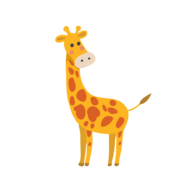
\includegraphics[width=0.25\textwidth]{images/giraffe_small}
\end{wrapfigure}

In my dream, there is the possibility of humankind to live in a world of peace through mutual understanding.
A world where we reached a deeper \textbf{understanding} of not only the other person but also of ourselves.
So often we disconnect so quickly from each other and ourselves, getting stuck in multiple layers of confusion and entangled stories.
The answer usually would be to go slower, to breathe \ldots

Yet, in my personal opinion, this is often not enough.
Not only do we need more tools, find solutions on a more technical level, but first and foremost the way we relate to language, people, and reality itself.
Many communication systems practice an outside-in approach --if there is even an inside existing-- where a certain mechanic is practiced on how to use words, yet not really feeling it.
Yes, people can tell me to use ``I-messages'' or to say ``thank you'', but it will be all worthless if it's not felt if it's not expressed while also deeply feeling the words.
This book's approach tries to also simultaneously use an \textbf{inside-out} approach, where once we establish a certain attitude, the ``correct'' words will come by themselves, and they will sound all natural and less like a programmed robot.

The way we talk, and use words, is the way we think.
And the way we think is the way we are.
By changing our way of talking, we change the way we are.
And that's why working on our communication skills is of the utmost importance.

\q{The ability to observe without evaluating is the highest form of intelligence.}{J. Krishnamurti}

It doesn't even end here, as to change our language, we need to change how we look at things.
At the core, we have our preconception of the world being separated in good and bad; the illusion of separation.
That there is a higher, authoritative power which holds the absolute wisdom of what's objectively right or wrong.
Once we let go of these fundamental concepts, but \textbf{see reality} without judging it, we open up a possibility to see reality in such a different way which can transform not only our but also the lives of others.

\section{Origins}\label{sec:origins}

\q{The good thing about reinventing the wheel is that you can get a round one.}{D. Crockford}

Everything has been basically already said, there is not much, or maybe even nothing to say anymore.
Sometimes we simply repackage what's already day to make it more fitting to the current times.
Having that said, the main sources of this book's approach are as follows:

\begin{itemize}
    \item \textbf{Non-Violent Communication}\footnote{Marshall Rosenberg himself, the inventor of NVC, considered the name to be a bit misleading but once it was out there, it couldn't be changed anymore.} makes up the foundation of this book, as most of it is based on NVC and its teachings.
    There are many classes and workshops given around the world, several books and videos exist, and there are even schools for children following this system's approach.
    \item \textbf{Radical Honesty} is a useful tool based on Gestalt Therapy, where we allow ourselves to fully own and express our judgments and projections, and find connection within ourselves and with others in a very raw and transparent form.
     By allowing ourselves to be fully seen, by holding space for the other and fully seeing him, we can establish a connection on a deeper level while dropping our masks and trying to be a ``nice, dead person''.
    \item \textbf{Circling} is less of a technical approach, but more a way to stay present, curious and mindful with the present moment of what is.
     We also try to stay focused on what is alive in the other person, asking ourselves how it would be to be that other person.
     Total awareness of our own inner sensations, staying grounded, and find the beauty also here in our human rawness.
    \item Schulz von Thun's \textbf{communication square} might look simple at first.
    However, once it is understood and applied in daily life, it can have a rather enlightening effect on the person.
    This is to be able to see reality a bit more clearly by having a more nuanced view on the layers of interpersonal communication.
    \item Byron Katie's \textbf{the work} is a small worksheet which allows us to see things from a different perspective.
    Seeing our own involvement in every interaction, letting go of blame and shame, and by seeing the full picture have some compassion with the other and ourselves.
    \item And of course many, many more which have \textbf{inspired}, supported, helped me to grow and improve my communication skills.
    Some teachers I have met personally, some I just read books about.
    People like Steven Covey, Dale Carnegie, Max Strom, Vera Birkenbihl et al.
\end{itemize}
